\documentclass[12pt,a4paper]{article}
\usepackage[utf8]{inputenc}
\usepackage[IL2]{fontenc}
\usepackage{amsmath}
\usepackage{amsfonts}
\usepackage{amssymb}
\usepackage{graphicx}
\usepackage{xcolor}
\usepackage{url}



%\title{Automatizovaná detekce a klasifikace jevů v časových řadách hydraulických sensorů}
\title{Automatized detection and classification of events in the time series of hydraulic sensors}
\author{Alexander Ma\v{c}ejovsk\'{y} \and \v{S}t\v{e}p\'{a}n Pardubick\'{y}}
\date{\today}

\begin{document}

%%\begin{titlepage}
%%    \centering
%%    \vspace*{2cm}
%%    {\huge\bfseries \maketitle}
%%    \vfill
   % \emph{Last edited on:} \today % Date will update automatically
%%    \vfill
%%\end{titlepage}

\maketitle % Insert title here

\thispagestyle{empty} % Remove page number from title page

\clearpage % Start the table of contents on a new page

\tableofcontents  


\newpage

\section{Introduction}

DHI is a water management company. Its portfolio includes water canals and pipelines with both fresh and waste water. The company uses physical models for predicting amount of flow in different locations. The quality of these models needs to be verified by empirical data collected by sensors situated directly in the canals and pipes which measure water level and velocity. Such measurements are then used for calculation of the water flow. Unfortunately, the sensors are not flawless as they can get clogged or otherwise corrupted by various objects flowing in the water. The fact a sensor reports faulty data can be usually detected by visual inspection of the resulting time series of its measurements. The goal of this project is to develop algorithms for automized detection and, ideally, correction of such measurement errors. The result should be a Python library encapsulating a suite of algorithms, designed to address data exploration, anomaly detection, visualization and correction of errors. This paper will summarize our work process and display our results to the reader. Given that the results of this project are expected to be implemented in practice, this report can be also used as a partial guideline.

\begin{figure}[ht]
  \noindent\makebox[\textwidth]{%
  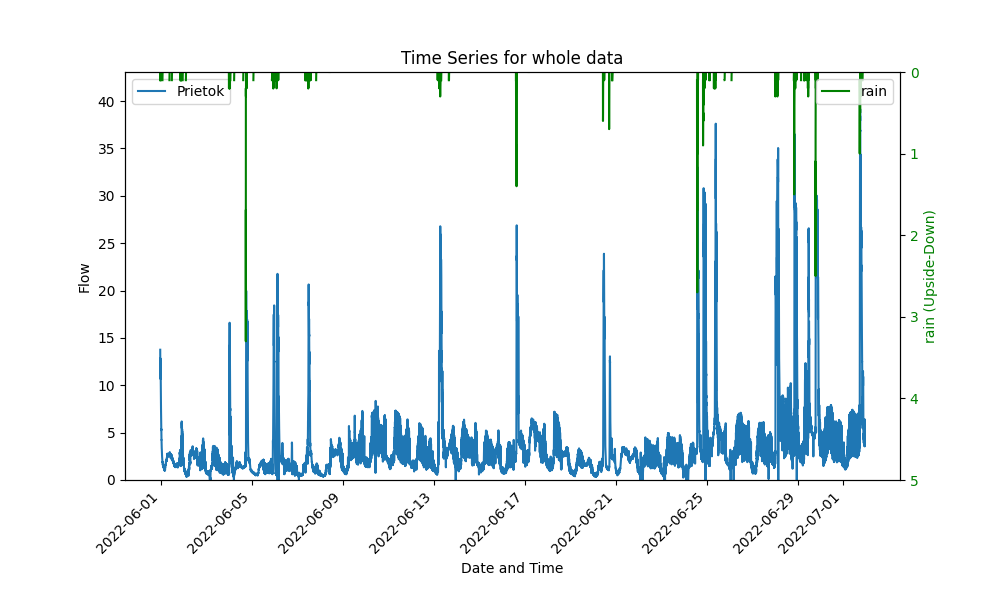
\includegraphics[width=1.4\textwidth]{Rain Dataset.png}}
  \caption{Example of a time series of flow in sewage pipe and measured precipitation (coming from MPO time series). It can be seen that the peeks in the flow coincide with rain.}
    \label{rain_data}
\end{figure}


We were given time series of the wastewater level, velocity and flow from various measurement stations in  sewage systems. This information is gathered by means of various sensors. These sensors can be prone to various types of malfunctions. They can get clogged, displaced or even break. It is important to be able to detect these forms of failures in the time series. The time series are, however, quite  volatile and noisy. They feature major upticks  coinciding with rain and natural daily cyclicity (peeks and increased volatility in the mornings and evenings when people tend to use shower, dishwasher etc.), see Figure \ref{rain_data} for an example.

The client wanted us to try to come up with an original solution to the problem not influenced by their own currently implemented methods. As such we were given little to no information as to what the errors look like and how to correct them. Due to neither of us having any expertise in the field of sewage management, our work should be seen as an attempt to innovatively explore an unknown field and develop new solutions. As such, our approach was to creatively utilize standard techniques for working with time series and create a framework for their further utilization, rather than using or developing overly complex methods.


\subsection{Task Description}
Our main task is to develop a Python library for automated detection and correction of  measurement errors in the time series of water velocity, level and flow. It can be broken down into the following steps:
\begin{itemize}
  \item Data exploration
  \item Definition and identification of events
  \item Correction of errors
  \item Development of Python library for handling of all of these steps
\end{itemize}

We were given several restrictions for how to proceed and what should our methods (not) use:
\begin{itemize}
    \item While the precipitation data is very useful for understanding involved time series, it cannot be accessed by the methods.
    \item Each time series should be viewed in isolation, data from different time series should not be directly used in the same process.
    \begin{itemize}
      \item{We should not fit a big model on all the data and then use it on individual series.}
      \item{We cannot utilize any relations between the series (for example to investigate several series in parallel).}
      \end{itemize}
      \item {We are not given any target data, that is labels for errors or non-defunct (corrected) series for testing the performance.}
      \item{While information for both water level and velocity is provided, the time series are to be investigated as univariate - the methods should be developed for the flow and then can be later tried on other variables.}
      \item {If possible, need for utilizing methods in the real-time or with the minimal delay should be considered. }
    
%Note that the lack of any labels is very prohibitive...
\end{itemize}


We managed to identify three broad types of apparent errors occurring in the data and propose their corrections depending on how long the respective sensor malfunction lasts. The actual implementation of the corrections has been in some cases  due to time limitations only partially accomplished. The following sections describe in greater detail the data we obtained for the task, the identification of potential errors, their corrections, further ideas and suggestions for future development, and brief description of the resulting Python library. 


\section{Data Exploration}
In this section we will focus on exploration and description of the data. We were provided with 43 csv files. After carefully examining them and extracting their contents we are able to gather information about 8 different measuring sessions taking place between years 2019 and 2023. These sessions span approximately 30 to 110 days and the observations come in two minute intervals. Each session thus contains approximately 22000 to 81000 individual data points. The extracted variables of interests are:\footnote{Note that we do not include the units in which the individual measurements come. This information was not shared with us by the client and cannot be easily deduced (the units seem to vary among individual time series).}
\begin{itemize}
    \item Time - date, hour and minute.
    \item Water level - measured by sensors.
    \item Water velocity - measured by sensors.
    \item Water flow - computed form water level, velocity and a known shape of the sewage pipe.
    \item Precipitation - measured by sensors, only contained in one (smallest) measuring session.
\end{itemize}
Several explanatory statistics for the datasets can be seen in the table \ref{tab: Basic exp 1}. The thorough exploration of these variables across the various measuring sessions laid the foundation for the development of solutions in the following chapters.

\begin{table}[h]
\centering
\begin{tabular}{rrrrrr}
  \hline
 &Start date & End date & Obs. count & Mean flow & Rain info \\ 
  \hline
    MP0 & 2022-05-31 & 2022-07-01 & 22319 & 3.60 & Yes \\ 
    MP1 & 2022-06-30 & 2022-10-20 & 80472 & 0.18 & No \\ 
    MP2 & 2022-06-15 & 2022-09-15 & 66254 & 0.0055 & No \\ 
    MP3 & 2021-01-26 & 2021-05-18 & 80749 & 0.036 & No \\ 
    MP4 & 2021-11-23 & 2022-02-28 & 69641 &  0.15 & No \\ 
    MP5 & 2021-06-28 & 2021-10-11 & 75470 & 0.0016 & No \\ 
    MP6 & 2022-11-13 & 2023-02-25 & 74904 & 0.13 & No \\ 
    MP7 & 2019-07-25 & 2019-10-25 & 66327 & 0.13 & No \\ 
    \hline
    &Min flow & Max flow& Std. of flow& Mean level& Mean velocity\\
    \hline
    MP0 &  0.00 & 39.15 & 4.18 & 192.84 & 0.26 \\ 
    MP1 & 0.052 & 1.75 & 0.12 & 0.24 & 1.06\\ 
    MP2 & 0.0013 & 0.40 & 0.010 & 0.073 & 0.18  \\ 
    MP3 & 0.00 & 1.33 & 0.031 & 0.12 & 0.81 \\ 
    MP4 & 0.067 & 1.20 & 0.062 & 0.17 &  1.30 \\ 
    MP5 & 0.0015 & 0.74 & 0.010 & 0.015 & 0.40 \\ 
    MP6 & 0.053 & 1.62 & 0.081 & 0.29 & 0.55 \\ 
    MP7 & 0.00 & 0.96 & 0.072& 0.31 & 0.62 \\
    \hline
   \end{tabular}
\label{tab: Basic exp 1}
\caption{Basic explanatory statistics for the provided time series.}
\end{table} 


\newpage

\section{Problem Formalization, Definitions and Notation}

We consider the following mathematical formalization of our problem. For given measurement location and variable of interest (flow, level or velocity) we represent the actual time series of measured variable by stochastic time series $\mathbf{Z} = \lbrace Z_t \rbrace_{t \in \mathbb{R}}$ for $Z_t:    (\Omega, \mathcal{F}) \mapsto (\mathbb{R}, \mathcal{B}(\mathbb{R})), \forall t \in \mathbb{R}$ being continuous real random variables. We assume the observed measurements come from  the stochastic time series with discrete time $ \mathbf{X} = \lbrace X_t \rbrace_{t \in \mathbb{Z}}$  with $X_t, t \in \mathbb{Z}$ being continuous real random variables defined on the same measurable space as $Z_t$. We then have 

\begin{equation}
    \label{eq:basic_eq}
    X_t = Z_t + \xi_t, \quad \forall t \in \mathbb{Z},
\end{equation}
where elements of $\lbrace \xi_t \rbrace_{t \in \mathbb{Z}} $ are again real random variables defined on the same measurable space. The latter thus represent imprecision of the sensor's measurements. We allow  $\mathbb{P}(\xi_t=0)>0.$

Observed measurements can be therefore understood as finite number of elements of a specific realization of the time series $\mathbf{X}$. We will denote them as $ \mathbf{x} = \lbrace x_t \rbrace_{t=0}^{T} =  \lbrace X_t(\omega) \rbrace_{t=0}^{T}$ for some $\omega \in \Omega$. Task of error identification can be then understood as determining  for $t=0,...,T$  when $\xi_t(\omega) \neq 0$ and for such cases the goal of the error correction task is then determining unknown values of $Z_t(\omega)$ based on observations of $X_t(\omega)$, which is thanks to the relation \ref{eq:basic_eq} equivalent with determining value of $\xi_t(\omega)$. 

We furthermore denote vector of the first differences of the observed measurements  as $ \Delta\mathbf{x}=  \lbrace\Delta x_t \rbrace_{t=1}^{T},$ that is 
$$ \Delta x_t = x_t - x_{t-1}, \quad t=1,...,T. $$

We used sample centred moving averages $MA_t(\mathbf{y}, W)$ and standard deviations $Msd_t(\mathbf{y},W)$ of given finite time series $\mathbf{y}$ with time window of length $W \in \mathbb{N}$, where 

$$ MA_t(\mathbf{y}, W) = \dfrac{1}{W}\sum_{\tau = -l}^{u}y_{t+\tau}  $$

$$ Msd_t(\mathbf{y}, W) = \sqrt{ \dfrac{1}{W-1}\sum_{\tau = -l}^{u}(y_{t+\tau} -MA_t(\mathbf{y},W) )^{2} }  $$
for $t=l,...,T-u$ and $ l = \lfloor \frac{W}{2} \rfloor, u = \lceil \frac{W}{2} -1\rceil. \lfloor  \cdot  \rfloor, \lceil  \cdot \rceil$ are lower and upper whole parts, respectively. For example, for $W=30$ we are summing over $\tau = -15,...,14$ and for $W=15$ over $\tau = -7,...,7.$


One of the main complications for examining behaviour of our time series is the fact it is significantly different in times when it rains as opposed to usual state of affairs. In some cases we found it useful to try to use measures which are estimated on the data which excludes rainy periods. For the lack of a more precise method, we use rough approximation of rainy periods as those for which the measured variable is above the $p^{th}$ quantile, where we use different values of $p$ for different purposes. Such approach is quite reliable in terms of false positives, that is, as far as we can judge, measured variables do not raise above certain levels unless it rains. Its weakness is that it is not able to capture periods when measurements are only at the beginning of their increasing trajectory caused by precipitations inflow. 

Most often we use this approach for calculation of what we refer to as (against rain-) \textbf{robust} \textbf{standard deviations}, which are calculated as the overall standard deviation of the time series after exclusion of the observations above the $p^{th}$ quantile, that is 
\begin{equation}
    \label{eq:rob_sd}
    \sigma_p(\mathbf{y}) = sd\lbrace y_t; y_t \leq q_p(\mathbf{y}) \rbrace =  \sqrt{ \dfrac{1}{T_p-1}\sum_{t= 0}^{T}(y_{t}\mathbf{1}(y_t \leq q_p(\mathbf{y})) -\overline{y_p} )^{2} }  
\end{equation}
with 
$$ \overline{y_p} = \dfrac{1}{T_p-1}\sum_{t= 0}^{T}y_{t}\mathbf{1}(y_t \leq q_p(\mathbf{y})) $$
and

$$T_p = \sum_{t= 0}^{T}\mathbf{1}(y_t \leq q_p(\mathbf{y})).$$
$q_p(\mathbf{y})$ denotes  $p^{th}$  sample quantile of the series $\mathbf{y}$ and  $\mathbf{1}(\cdot)$ is a zero-one binary indicator of the truthfulness of given condition. 

We often speak of the \textbf{groups} of observations. By this we mean uninterrupted series of successive observations with some characteristic. For example, observations between times $t_1$ and $t_2$ constitute group of zero observations if $x_t=0, \forall t \in \lbrace t_1, ...,t_2 \rbrace$ and $x_{t_1-1}, x_{t_2+1} \neq 0$.

Following methods rely on adjustable parameter values. In order to automatize implementation of the methods we always provide a default value for each parameter, which is denoted in text as $parameter=number$ at the first mention of each parameter. See also Table \ref{tab:default_vals} for their summary. For easier reference we also denote parameters by the \textcolor{blue}{blue} font.


\newpage
\section{Identified Events}

Two main approaches to the identification of errors were taken. First, we tried to use statistical methods for unsupervised classification such as Autoencoder and K-Means clustering. While these methods showed some interesting results, it was difficult to fine-tune them due to lack of target examples, see Section \ref{sec:other_sugg} for more information. The second approach was to visually inspect provided time series, subjectively identify suspicious observations and devise heuristic  rules for their automatic detection. The latter approach was supplemented by  consultations with the DHI experts and, based on the consultations and our own opinion, seemed to work satisfactorily well. Due to time limitations we therefore decided to focus solely on the second approach. It needs to be noted that the following methods were devised for use on the most general cases, as more  refined adjustments of the methods was not possible due to time limitations. However, the implemented code solution provides great amount of flexibility in the actual application of the methods on individual special cases, see Section \ref{sec:pyth_lib} for more details.

Given that one of the considerations of the project is to develop methods which can work in the real-time or with minimal delay, we also provide brief discussion of data requirements for classification of each of the error types.



\subsection{Constant and Zero Values}

\begin{figure}[htbp]
    \centering
    \begin{tabular}{c}
        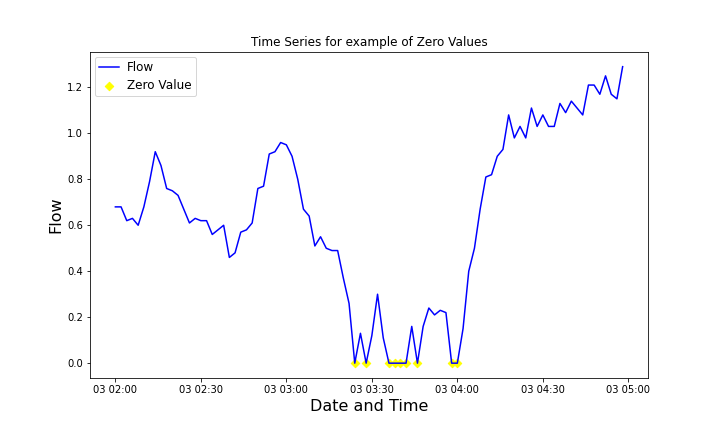
\includegraphics[width=0.99\linewidth]{zeros_ex.png} \\
        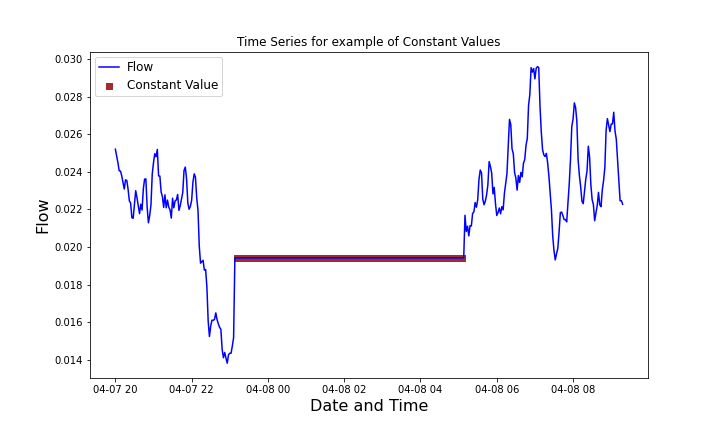
\includegraphics[width=0.99\linewidth]{const_ex.png} \\
    \end{tabular}
    \caption{Examples of Zero and Constant Values errors.}
    \label{fig:zero_const_ex}
\end{figure}

One of the most evident errors happen when a sensor reports zero values or is stuck at reporting some other constant value over a prolonged time horizon. In some rare cases sensors even reported negative values. Although there exist reasons for why some of such measurements might be legitimate, neither of these cases is generally expected and we thus chose to classify them as an error. 
We denote as Zero Values both  observations of zero values and those rare cases when observations are negative, that is $x_t \leq 0$. 

Identification of Constant Values happens in two steps. In the first step, we identify as possible Constant Values  those observations which are the same as their neighbouring past and future observations, i.e. observation at time $t$ is constant if $x_{t-1} = x_t = x_{t+1}$. Note that in such a case observations at times $t-1$ and $t+1$ are not classified as constant observations unless they themselves satisfy analogous condition. Technically, this classification is done by identifying zero moving standard deviation of the main variable  with window 3,

$$ Msd_t(\mathbf{x},\textcolor{blue}{W_0} ) = 0 $$
with $\textcolor{blue}{W_0}  = 3$. However, isolated or small groups of (non-zero) constant observations  can be either ignored without any practical impact on the quality of the empirical data or might be even caused by rounding of the temporary stable correct measurement series. In the second step, we thus recognize candidates from step 1 as Constant Values only if they are part of the group of candidates in which \textbf{there is at least} $\mathbf{\textcolor{blue}{tol\_const}  = 5}$ \textbf{of them in succession,} otherwise they are ignored as regular observations.  Setting either of parameters $\textcolor{blue}{W_0} $ and $\textcolor{blue}{tol\_const} $   to some higher then default value would result in a less strict error classification and less number of  identified Constant Value errors.  

\textbf{Data requirements}: Zero Values can be identified immediately while with the default parameters, there is delay of  6 periods ($\textcolor{blue}{tol\_const}+\lceil \frac{\textcolor{blue}{W_0}}{2}-1 \rceil$) for identification of the first Constant Value error in the given group of Constant Values.




\subsection{Heightened Volatility}

\begin{figure}[htbp]
    \centering
    \begin{tabular}{c}
        \includegraphics[width=0.99\linewidth]{calm_ex.png} \\
        \includegraphics[width=0.99\linewidth]{volatile_ex.png} \\
    \end{tabular}
    \caption{Examples of relatively calm and unusually volatile flows. Width of the robust standard deviation bounds (black lines) are the same in both plots and serve as an anchor for comparison. }
    \label{fig:volatile_ex}
\end{figure}

Sometimes, time series of our main variable is suspiciously more volatile than at other comparable times. This is characterized by large  up and down jumps of the measured series, that is volatility is heightened also in the first differences of the series. Possible cause of this behaviour might be presence of large chunks of waste in the water which disturb sensor's measuring technique, although DHI experts would prefer to simply receive warning about such events instead of automatically considering it as an error. An example of such behaviour can be seen in Figure \ref{fig:volatile_ex}. The upper panel shows relatively typical behaviour of the water flow in certain location during one day. The lower panel shows water flow time series from the same location on a different day. Heightened volatility is apparent especially if we pay attention to the robust standard deviation bounds, which have the same width in both panels, and compare them to bounds created by moving standard deviations (with window of length 30 periods). In the former case, the latter bounds are much more narrow than the robust bounds but they become as wide or even more so in the lower panel. 

The heuristic rule for identification of heightened volatility is based on the high values of moving standard deviations. However, we first had to determine whether to consider standard deviations of the main variable or of its first differences. Volatility of the first difference is similar to direct volatility but the former is too sensitive to transitions of the main variable to different levels, for example due to incoming precipitations. Using first differences led to somewhat fewer cases of such intuitively undesired, and hence false positive, identifications.  

We therefore chose to consider volatility of the first differences for the classification purposes. We do this in two steps. First, we identify suspicious observations with high values of moving standard deviation of its first differences,

$$ Msd_t(\mathbf{\Delta x},\textcolor{blue}{W_2}) > K $$
where we chose window  \textcolor{blue}{$W_2$}$ = 30 $ observations corresponding to the 1 hour period.  Our aim is to consider medium-term volatility and we consider this as a natural choice for medium-term interval. Threshold $K$ is determined as the \textcolor{blue}{$c_2$} $=1$ multiple of the overall standard deviation for the observations below the $\textcolor{blue}{p_1} = 0.7^{th}$ quantile of the first differences, that is of the robust standard observation (see equation \ref{eq:rob_sd}),
$$ K = \textcolor{blue}{c_2} \cdot \sigma_{\textcolor{blue}{p_1}}(\mathbf{\Delta x}).$$
 Choosing lower $\textcolor{blue}{p_1}$ or $\textcolor{blue}{c_2}$ would lead to  higher sensitivity to and more detected case of heightened volatility and vice versa. Motivation behing these choices is that the overall standard deviation is a natural  threshold for determining what are normally occuring variations as opposed to unusually high ones. However, rain makes the series more volatile than it is in its usual state, which is why we use robust standard deviations instead of the simple ones. Meanwhile,  $\textcolor{blue}{c_2}$ serves as a refinement parameter.

This first step makes decisions about individual observations. However, we deem that detecting high volatility as the result of sensor's malfunction makes practical sense only for larger groups of successive observations rather than individual ones. Therefore, there are two possible problems we need to further consider. First, there might be short-term breaks between two longer-term volatility periods due to moving standard deviation getting temporarily slightly under the chosen threshold. On the other hand, there can be borderline cases from the opposite direction, when moving standard deviations get for a short time slightly above the threshold but then recede back below it again. This makes classification by the first step occasionally undesirably noisy.

We deal with this in the second step, in which we  identify groups of high volatility observations (successive periods in which high volatility is recognized) and decide that  if there are two such neighboring groups separated by less then $\textcolor{blue}{tol\_vol_1} = 5$ non-volatile observations we merge them by classifying observations between them as high-volatility observations as well. Second, if a group of highly volatile observations, even after previous merging,  has less than $\textcolor{blue}{tol\_vol_2} = 5$ members, we deem it as a false signal and do not categorize these observations as volatile.

\textbf{Data requirements}: Calculation of moving standard deviations require $\lceil \frac{\textcolor{blue}{W_2}}{2}-1 \rceil$ future observations, i.e. lead to delay of 14 periods when  the default parameter values are used. Calculation of threshold $K$ requires the whole history of the data and can be dynamically redone immediately after obtaining a new observation. If the past history of the series is not directly available the implemented solution provides option to input customized value of the threshold $K$, for example based on the history of the series from indirect sources or as some expertly determined value.

\subsubsection{Volatility Due to Rain}
When it is raining we consider it natural and unsurprising that volatility is relatively high. We thus try to recognize when this happens due to influx from precipitations. As mentioned previously, rain is usually accompanied by heightened level of the measured variables (directly, not their first differences), hence we classify observation $x_t$ as being volatile due to rain if it was classified as volatile and in addition it satisfies that 

$$    MA_t(\mathbf{x},\textcolor{blue}{W_3}) \geq q_{\textcolor{blue}{p_2}}(\mathbf{x}).  $$
For default values we chose $\textcolor{blue}{p_2} = 0.9$ and $\textcolor{blue}{W_3} = 5$. Given time window was chosen by considering that, first, we are interested in the more immediate characteristic of the series while, second, rain is not a sudden event and neighbouring observations can give valuable signal about wether it is raining or not. Note the difference between $\textcolor{blue}{p_1}$ and $\textcolor{blue}{p_2}$ due to latter relating to the main variable while the former to its first differences.

We furthermore perform the same kind of grouping as for the general high volatility described above, this time with $\textcolor{blue}{tol\_rain_1} = 5$ for elimination of gaps between groups of volatility and $\textcolor{blue}{tol\_rain_2} = 10$ for elimination of too small groups of volatility.

Figure \ref{fig:rain_ex} shows examples of observations classified as volatile and as volatile due to rain based on the algorithms described above.

\textbf{Data requirements}: This category is subset of the heightened volatility, so the same requirements as above hold. Additionally, we need to calculate moving average with the window $\textcolor{blue}{W_3}$, but this window is in the default setting and by our thinking expected to be smaller than the one required for the heightened volatility identification. We use the whole history of the data for calculating $\textcolor{blue}{p_2}^{th}$ percentile of the main variable. For this the same comment applies as for the threshold $K$ above. 

\begin{figure}[htbp]
    \centering
    \begin{tabular}{cc}
        \includegraphics[width=0.99\linewidth]{vol_class_ex.png} \\
        \includegraphics[width=0.99\linewidth]{rain_vol_class_ex.png} \\
    \end{tabular}
    \caption{Examples of identified suspicious volatility and volatility due to rain events. Examples of  isolated outliers can be also seen.}
    \label{fig:rain_ex}
\end{figure}

\subsection{Outliers}
Not too  uncommon occurrence are measurement values which seem odd compared to nearby past and future values, see for example Figure \ref{fig:rain_ex}. $x_t$ is identified as an outlier if the measured value jumped by high margin up and then immediately fell by high margin down, or vice versa, fell and than risen back again, i.e.
$$ \Delta x_t > T_t \qquad \text{and} \qquad \Delta x_{t+1} < -T_t $$
or analogously with $\Delta x_t$ and $\Delta x_{t+1}$ switched around, respectively.

We judge whether such jumps are large or not based on the current volatility of the first differences of the series. Threshold $T_t$ is hence dynamically based on the moving standard deviation of the first differences of the main variable as 
$$ T_t = \textcolor{blue}{c_1} \cdot Msd_t(\mathbf{\Delta x},\textcolor{blue}{W_1}). $$
As default values we chose  window $\textcolor{blue}{W_1} = 30$ for measuring medium-term volatility and multiplier  $\textcolor{blue}{c_1} = 2.5$. The latter is inspired by the standard rule of thumb which says (inspired by characteristics of normal distribution) that approximately $95\%$ of observations are within the $\pm 2$ standard deviations boundary around the mean. We decided to be even more strict and use $\pm 2.5$ boundary, which in case of normal distribution approximately corresponds to the $99\%$ confidence bound. Note however, that this is just a rule of thumb, we do not make specific assumptions about the distribution of our variables of interest. 

\textbf{Data requirements}: Calculation of moving standard deviations leads to delay of $\lceil \frac{\textcolor{blue}{W_1}}{2}-1 \rceil$ periods, that is 28 minutes in the case of default value and 2 minutes observation periodicity. 

\subsection{Prolonged Drops}
Lastly, we aim to detect additional event - prolonged drops\footnote{Prolonged drops detection was suggested by the client late in the development and is currently only in its first draft. The provided datasets do not include many good examples of this error. Corrections of the prolonged drops have also not been developed.}. Sometimes a drop in the flow is not immediately followed by a bounce-back and the series takes more time to return to previous levels.
For an observation to be classified as prolonged drop, it needs to meet 3 requirements:
\begin{enumerate}
    \item Drop
    \begin{itemize}
        \item A significant drop in the main variable needs to occur. We detect this by $x_t$ being lower then average of preceding \textcolor{blue}{$W_4$} values by a certain threshold (defined similarly as in outlier case):
        \[
         x_t < \frac{1}{\textcolor{blue}{W_4}}\sum_{\tau=1}^{\textcolor{blue}{W_4}}x_{t-\tau} -T_t, \qquad T_t = \textcolor{blue}{c_3} \cdot Msd_t(\mathbf{\Delta x},\textcolor{blue}{W_1}).
        \]
        \textcolor{blue}{$c_3$} is set to 2 by default, \textcolor{blue}{$W_4$} to 3 and \textcolor{blue}{$W_1$} to 30 is the same parameter which was used for detection of outliers.
    \end{itemize}
    \item Prolonged duration
    \begin{itemize}
        \item All of the following $\textcolor{blue}{n_{fol}}$ observations ($x_{t+1}\dots x_{t+\textcolor{blue}{n_{fol}}}$) need to be bellow a threshold defined by the preceding value  $x_{t-1}$:
        \[
        x_{t+i} < \textcolor{blue}{c_4} x_{t-1}, \qquad \forall i \in \{1,\dots, \textcolor{blue}{n_{fol}}\}.
        \]
        $\textcolor{blue}{n_{fol}}$ is set by default to 3 and \textcolor{blue}{$c_4$} to 1.
    \end{itemize}
    \item Drought
    \begin{itemize}
        \item In the presence of rain among the preceding observations, prolonged drops are a natural thing to occur and should not be classified as errors. We check whether any of the previous \textcolor{blue}{$n_{prev}$} (set to 10 by default) observations were classified as "rainy", that is if they were above $\textcolor{blue}{p_2}^{th}$ quantile. If any of them were, then the observation cannot be classified as a prolonged drop.
    \end{itemize}
\end{enumerate}

Note that only the first observation (the observation where the drop occurred) is classified. Example of detected prolonged drop can be seen in the figure \ref{prol_drops}.

\textbf{Data requirements}: Determination of rainy observations requires calculation of $\textcolor{blue}{p_2}^{th}$ quantile of the whole series, see comments about data requirements of volatility identification above. We also need $\max\{\lceil \frac{\textcolor{blue}{W_1}}{2}-1 \rceil$ , $\textcolor{blue}{n_{fol}}\}$ future observations, that is in default case we could identify prolonged drops with 28 minutes delay.


\begin{figure}[ht]
  \noindent\makebox[\textwidth]{%
  \includegraphics[width=1.4\textwidth]{prol_drops.png}}
  \caption{Example of a classified prolonged drop (labeled prol\_down). Note the difference between prolonged drop and outlier.}
    \label{prol_drops}
\end{figure}




\begin{table}[h!]
    \centering
\begin{tabular}{|cc|cc|cc|}
    \hline
    parameter & value & parameter & value & parameter & value \\
    \hline
    $W\_0$& 3 & $c_1$ & 2.5 & $tol\_const$& 5  \\
    $W\_1$& 30 & $c_2$ & 1 & $tol\_vol_1$ & 5 \\
    $W\_2$ & 30 & $p\_1$ & 0.7 & $tol\_vol_2$ & 5 \\
    $W\_3$ & 5 & $p\_2$ & 0.9 & $tol\_rain_1$ & 5 \\
    $n_{prev}$ & 10 & $n_{fol}$ & 3 & $tol\_rain_2$ & 10 \\
    $W\_4$ & 3 &  $c_3$ & 2 &  $c_4$ & 1\\
    \hline
\end{tabular}
\caption{Default parameter values.}
    \label{tab:default_vals}
\end{table}


\newpage
\subsection{Hierarchy of Events}

We categorize each observation to just one group. Since an observation can sometimes satisfy conditions for multiple categories we set classification priority as follows (from the most preferred category to the most overwritten):

\begin{enumerate}
    \item Outliers
    \item Prolonged drops
    \item Zero values
    \item Volatility due to rain
    \item General volatility
    \item Constant values
\end{enumerate}

For example, an outlier satisfying conditions for prolonged drops category will be classified as an outlier and series of zero values will be classified as such, not as constant values. Observations which do not belong to any of these categories are considered to be accurate, i.e. satisfying $\xi_t(\omega) = 0$.






\newpage
\section{Corrections of Errors}

The most important factor for choosing the method for correction of errors is the length of the corrected sensor malfunction. For short-term malfunctions of less than 8 periods we expect the results of any standard reasonably applied method would not differ much from the smoothed values of the original time series based on the accurate observations surrounding the  group of faulty observations which is being corrected. For longer malfunctions, choice of the method becomes significant for the quality of corrections. Especially for malfunctions lasting several hours or even days there is an opportunity for examining and using cyclicity present in the data for making predictions more akin to standard behaviour of the underlying time series. We chose to differentiate between short-term (less than 8 periods), medium-term (between 8 and 60 periods) and long-term (more than 60 periods) malfunctions. Exception is the case of heightened volatility, which is in all cases corrected by simple smoothing by centered moving averages. The following subsections provide details.



\subsection{Volatility}

As mentioned in the previous section, heightened volatility might be caused for example by large elements flowing in the water and disturbing sensor's ability to use reflections of radar or sonar signals for measuring velocity and level of the water.  In any case, we assume such disturbances would lead to zero-mean errors. Given the nature of the underlying physical processes we naturally assume that the measured time series are characterized  by positive and rather high autocorrelation, which is also apparent from their graphs. We thus use simple smoothing by moving averages for clearing the data from the noise produced by aforementioned disturbances, that is 

$$\hat{Z_t} = MA_t(\mathbf{x}, \textcolor{blue}{W_{vol}}),$$
where $ \hat{Z_t}$ stands for the corrected observation, that is estimate of the true value of the main variable $Z_t$ at time $t$. Parameter \textcolor{blue}{$W_{vol}$} is again adjustable with the default value 5. DHI experts have not considered heightened volatility as priority problem and we thus assume that to significant extent it is a true characteristic of the underlying variable as opposed to being mostly consequence of the errors. The default value leads to smoothed series which nevertheless relatively closely follows short-term trends and changes in the data while decreases volatility of the first differences and eliminates huge jumps. Choice of larger window would lead to smoother series which less faithfully copies the original observations. This would be appropriate for cases when it is supposed the underlying variable is actually quite stable and volatility is caused mostly by the measurement disturbances. Figure \ref{fig:short_corr_ex} provides, among others, a short example of how volatility corrections look like.

Regarding heightened volatility due to rain, we consider this to be a natural consequence of the underlying physical factors and regard such observations as accurate without the need for corrections.
 

\subsection{Short Term Errors}


\begin{figure}[htbp]
    \centering
        \includegraphics[width=0.99\linewidth]{short_corr_ex.png}        
    \caption{Example of corrections for short-term events and volatility. }
    \label{fig:short_corr_ex}
\end{figure}

As already discussed we consider errors to be short-term if the group of successive errors has less than 8 members.
Outliers are by definition always lasting only one period. We again use the assumption that the underlying time series shows high degree of positive autocorrelation and its actual value at time $t$ can be quite precisely detected from its values at times $t-1$ and $t+1$. We do not apply any weighting but simply set

$$\hat{Z_t} = \dfrac{x_{t-1} + x_{t+1}}{2}.$$
As noted in the previous section, we have not developed methods for correction of prolonged drops. The remaining errors to discuss are zero and constant values. 

Both of these events are corrected by using

$$\hat{Z_t} = MA_t(\mathbf{x}, \textcolor{blue}{W_{zero}})$$
where the default value of \textcolor{blue}{$W_{zero}$} is 15. Given short time span we assume good fit of corrections is not significantly dependent on the choice of specific method as long as it is not absolutely unreasonable one. Due to aforementioned principles of high autocorrelation and assumption of zero average error we consider moving averages as an easy and adequate solution for this case.


\subsection{Medium Term Errors}
\textbf{Note:} Due to time limitations the implementation of the medium term errors corrections has been accomplished only partially, on chosen exemplary cases. Full automation is in the stage of planning.

We define medium-term errors as those for which groups of successive errors have between 8 and 60 members. For construction of corrections we examined various models from ETS and ARIMA families. Due to small periodicity of observations, which is 2 minutes, it was impractical to consider seasonality component in ETS models estimated on the original data. We thus focused on ARIMA models. Generally, our  recommended approach would be to choose ARIMA parameters by minimizing Akaike Information Criterion inside a finite grid of possible parameter values. However, given the following considerations, we settled on a general choice of ARIMA(3,1,2) model.

This was done because we do not estimate one ARIMA model for the whole series but for each error group we chose to select 200 observations prior to the start of the error event  as the estimation sample.  Given that this leads to estimation of a new ARIMA model  for each group of medium-term errors, performing search of optimal parameters for each of them would be computationally prohibitive. The choice of (3,1,2) ARIMA parameters has been done due to time limitations rather arbitrary based on a few exploratory experiments.

%This was done because we do not estimate one ARIMA model for the whole series but for each error group we chose to select 200 observations prior to the start of the error event  as the estimation sample. Moreover, since we typically know the history of time series both before and after the error event took place we can estimate for the same error event one ARIMA model from the prior observations and, analogically, reverse the time direction and estimate another ARIMA model based on the later observations.  Given that this leads to estimation of two  new ARIMA models for each group of medium-term errors, performing search of optimal parameters for each of them would be computationally prohibitive. The choice of (3,1,2) ARIMA parameters has been done due to time limitations rather arbitrarily based on a few exploratory experiments.

Formally, our models have thus the form

$$ \Delta Z_t = \rho_1 \Delta Z_{t-1} + \rho_2 \Delta Z_{t-2} +\rho_3 \Delta Z_{t-3} + \epsilon_t +\phi_1 \epsilon_{t-1} + \phi_2 \epsilon_{t-2} $$
for times $t$ in the vicinity of the given error event, where we assume that terms $\lbrace \epsilon_t \rbrace$ come from the white noise process WN(0,$\sigma ^{2}$). For estimation purposes we use observed values $\mathbf{x}$, respectively $\mathbf{\Delta x}$ instead of $\mathbf{Z}$ and  $\mathbf{\Delta Z}$.
We create corrected values as predictions from this model,

$$\hat{Z_t} = \hat{Z}_{t-1} + \hat{\Delta Z_{t-1}} = \hat{Z}_{t-1} + \hat{\rho_1} \hat{\Delta Z_{t-1}} + \hat{\rho_2} \hat{\Delta Z_{t-2}} +\hat{\rho_3} \hat{\Delta Z_{t-3}} $$
with $\hat{Z}_{\tau}$ and $\Delta\hat{ Z_{\tau}}$ denoting either observed values $x_{\tau}$,  $\Delta x_{\tau}$ at time $\tau$ if $\tau$ refers to the ARIMA model estimation sample or predictions if $\tau$ refers to  period corresponding to one of the corrected errors.



%\textcolor{green}{statistical models, combination of forward/backward-looking predictions by exponential weighting, calculation on accurate or already corrected data only}



\subsection{Longer Term Errors}
\textbf{Note:} Due to time limitations the implementation of the longer term errors corrections has not been accomplished and the following explains the plans for it.

Main goal for correcting longer-term malfunctions is to utilize cyclicality of the underlying time series. Given their nature - water use tends to vary with the amount of human activity, which is connected to the time of the day, working days, special events etc. -  we determined to detect cyclical components on the level of hours of the day, individual weekdays, and  weekends. We did not expect presence of cyclicality on smaller time scales than that, which is the reason why we did not deem it practical to utilize this approach for short or medium term malfunctions.

For modelling cyclicality, we chose a simple dummy variables approach. As in the previous cases, only data of accurate or already corrected observations is used for estimation. We furthermore eliminated from the underlying time series upper 10th quantile as a rough attempt to clean the data of the rain, which might severely bias our estimates of typical (non-rainy) cycles. The cyclical components were then estimated by the OLS method applied on the model.
The dummy variables parameterize individual hours of the day and day of the week (note that the library supports additional models and even the ability to utilize external ones). The model also includes interaction between those two:

\begin{multline}
    Z_t = \sum_{i} \beta_i \mathbf{1}("t\text{ is in $i$-th hour}") + \sum_{j}\beta_j \mathbf{1}("t\text{ is in $j$-th day of the week}") \\
    + \sum_{i}\sum_{j} \beta_{ij} \mathbf{1}("t\text{ is in $i$-th hour}")\mathbf{1}("t\text{ is in $j$-th day of the week}")+\epsilon_t,
\end{multline}
where $\epsilon_t$ is the error term. Observed values $\mathbf{x}$ are used for estimation instead of $\mathbf{Z}$. The baseline cyclical adjustments are then computed as predictions by the model $\hat Z_t$ minus the average flow $\bar x_n$:
\[
cor_t' = \hat Z_t - \bar x_n.
\]
These baseline adjustments are then smoothed-out by simple centered moving average of length 7. We get smoothed adjustments $cor_t$.

%\textcolor{red}{Alex: zbytek tohoto textu mi moc nedává smysl, jak jde dohromady s napočtenými korekcemi (zkorigovanou řadou). "Odsezóněná" řada vznikne odečtením $cor_t$ a naopak statická řada se opravuje přičtením této složky.}
%The corrected time series is calculated by using predictions/fitted values of the cyclical model.
%In order to ensure smooth connection of corrections to the past and future accurate observations at the borders of the errors group, we again create two sets of predictions which we then convexly combine as in the case of medium-term corrections. The first set of predictions consist the cyclicality model predictions shifted up or down by a constant so that  the first predicted value is equal to the last accurate observation before the malfunction began. The second set of predictions is shifted in analogous manner so that its last predicted value is equal to the first accurate observation after the corrected malfunction ended.  

\subsection{Order of Corrections}

We aim to base our corrections on the accurate observations, that is observations which were not classified as errors or which had been already corrected. This means that when calculating measures used for error corrections we ignore data deemed as faulty (technically, we set them to NA values). Exceptions are correction of heightened volatility, for which we smooth the values of original observations by applying moving averages on the surrounding observations, which are typically also highly volatile, and outliers, which are dependent only on immediately preceding and following observations. We are not aware of any case where the latter would be in such cases classified as an error other than highly volatile.

For our approach the order in which corrections are undertaken plays an important role. We first correct outliers. This is followed by smoothing of the highly volatile observations. After that, we subsequently correct all short-term, medium-term and, finally, long-term errors. Correction of zero values takes precedence over correction of constant values. Otherwise, groups of errors are corrected from the oldest to the newest.  




\newpage
\section{Performance Evaluation}
%\textcolor{red}{TBD:no target $\Rightarrow$ not clear how to do this, but detection of events done expertly with the help of consultations,  basic idea for evaluation of corrections could be that no (only few) errors should be detected in already corrected time series }

In this chapter, we provide a concise exploration of the performance evaluation for our methods. It is important to note the inherent challenge in measuring performance due to the absence of labeled data or a well-defined description of the desired outcome. Instead of proposing a definitive measurement approach, we offer a brief overview of potential avenues for conducting performance evaluations in the future:
\begin{itemize}
    \item Qualitative assessment
    \begin{itemize}
        \item One approach  to evaluate performance is through qualitative assessment. This involves visually inspecting the output of our methods and subjectively gauging their appropriateness and effectiveness. Note that this should be preferably done with different data, than the one used to develop the methods.
    \end{itemize}
    \item Performance metrics utilizing labeled data
    \begin{itemize}
        \item If the labeled data were provided, then the performance evaluation would be straightforward. Metrics such as accuracy could be effortlessly calculated for event classification, providing a clear assessment of the model's classification accuracy. Additionally, evaluating the correctness of corrections would be straightforward, with measures like root mean square error easily computed when presented with the desired cleaned time series. This structured approach not only facilitates quantitative assessments but also allows for robustness testing, enabling us to evaluate the performance of our methods in extreme cases.
    \end{itemize}
    \item Performance check on cleared series
    \begin{itemize}
        \item If we were given cleared time series data instead of labeled data (that is time series containing no errors), we would anticipate that the methods should not detect any errors. Verifying and evaluating this expectation could be done easily.
    \end{itemize}
\end{itemize}




\newpage
\section{Other Suggestions and Ideas}\label{sec:other_sugg}

In this section we would like to briefly discus some approaches we tried, but which ultimately did not lead to the desired results.


\subsection{Unsupervised learning}

Unsupervised learning is a branch of machine learning where the algorithm is provided with input data without explicit labels. Unlike supervised learning, where the algorithm is trained on labeled data with clear input-output pairs, unsupervised learning involves working with unlabeled data to discover patterns, relationships, or structures within the information. This absence of requirement of labeled data is what led us to explore some methods belonging to the realm of unsupervised learning. 

\subsubsection{K-Means Clustering}
K-Means clustering is based on  assigning observations to categories based on their spatial location within the space of features. For given number of categories and given metric for measuring distance between numerical vectors, the algorithm finds a center for each category and assign observations to the category of which center it is closest to. The centers are assigned with the goal of minimizing the sum of final distances of individual observations to the center of their category. This algorithm requires initial assignment of centers and its results are sensitive to it, which is why its calculation usually involves iteration through multiple random initial settings and final choice of the result which has the minimal final sum of distances.

In our case, we chose the standard Euclidean metric and tried to use the algorithm on standardized features based on the water flow, such as moving averages and standard deviations of different window width, estimates of the time derivation of the series based on polynomial regression, first and second differences of the flow, time index and various others. We considered different numbers of groups between 2 and 8. For different interpretation approach we also tried to use the algorithm on the principal components of the engineered features. 

While this led to many interesting results, in some of which we could recognize events like heightened volatility or rain, lack of clear interpretation and clear-cut way of fine-tuning the method for automatized use led us to abandon this approach.

\subsubsection{Autoencoder}
An autoencoder is a type of artificial neural network used for unsupervised learning and dimensionality reduction. Its architecture consists of an encoder and a decoder, and it aims to learn a compressed representation of input data. The algorithm can identify anomalies by detecting deviations between the input data and the reconstructed output. 

We tried to utilize some autoencoder methods. The results were, however, rather poor. The algorithms could easily detect rains, as major sources of "unexpected" flow, but performed rather poorly otherwise. After a brief trial, these algorithms were quickly dismissed.

It is possible that good outcomes could be achieved by this class of algorithms, but it would require adept feature engineering and a better understanding of the subject matter, necessitating help of experts.


\newpage
\section{Python Library} \label{sec:pyth_lib}
% \textcolor{green}{TBD:brief summary of what the resulting library can do (plotting - multiple series and measures, results, serially broken down to smaller periods; classification, corrections; everything automatized by using default values but each step can be customized at the level of individual time series or even individual groups of events), + link to the github page (we should probably restrict it with a password)}

This chapter aims to provide a brief summary of capabilities of the resulting python library we created. Note that this is not intended as exhaustive description - the code is well written and includes a plethora of comments and docstrings to describe the usage of contained classes and functions. The code can be viewed in the following GitHub repository: 
\url{https://github.com/macejova/Ecox-seminar-project}, where the library resides in the file \textit{functions.py}. The functionalities of the library contain among others:
\begin{itemize}
    \item Data loading methods
    \begin{itemize}
        \item Loading, cleaning and merging time series.
        \item Handling of missing values.
        \item Folder scraping method for loading large amount of datasets.
    \end{itemize}
    
    \item Time series class (TS\_Class)
    \begin{itemize}
        \item The main class for working with time series.
        \item Other functions are implemented to work with this object.
    \end{itemize}

    \item Data Explorer Class (DataExplorer)
        \begin{itemize}
            \item Automation of working with multiple TS objects at once.
        \end{itemize}

    
    \item Plotting
    \begin{itemize}
        \item Highly customizable functionality for visualizing the data.
        \item Ability to display various statistical measures such as moving averages.
        \item Possibility to plot multiple variables at the same time.
        \item Flexible length of the time interval displayed.
        \item Displaying of the classified events. Easy comparison of the original and corrected time series.
    \end{itemize}
    
    
    \item Cyclicity adjustment
    \begin{itemize}
        \item Measuring of the cyclical component.
        \item (Smoothed) elimination of cyclical component.
    \end{itemize}
    
    \item Event classification
    \begin{itemize}
        \item Classification of the various events.
        \item Highly adjustable to fit the current problem.
    \end{itemize}
    
    \item Error correction
    \begin{itemize}
        \item Corrections of the classified events based on the grouping of successive observations of the same category and length of these groups.
        \item Choice of which categories or even specific groups of observations should or should not be corrected.
        \item Option to adjust values of correction parameters according to the need of specific problem at the level of the whole time series or of individual groups of errors.
    \end{itemize}
    
\end{itemize}

The entire library is written in a nonrestrictive manner. All of the functions are defined with default parameter values carefully set to perform well on our task and data. This provides high level of automatization. On the other hand, the parameters can be customized in a wide variety of ways, at the level of individual time series or even individual group of events. Functions are often written in a way which supports easy inclusion of external methods.





\newpage
\section{Utilized Python libraries}


In this section we give a quick summary of the most important Python libraries we used in the task. In addition, library datetime was used for basic handling of dates in datetime format, and Python built-in libraries warnings and os  were used for handling warning messages and  local repository files, respectively. For the sake of version control, Table \ref{tab:versions} provides list of versions of the used libraries with which the project was developed.  



\begin{table}[h!]
    \centering
    \begin{tabular}{|c|c|c|c|}
    \hline
        Library &  versions &  Library & versions  \\
        \hline
        NumPy & 1.18.5 & Statsmodels & 0.12.2 \\
        Pandas & 1.2.4  & Scikit-learn & 0.23.2 \\
        Matplotlib & 3.3.2 & warnings, os (Python) &  3.8.8 \\
        datetime & 3.3.2 &  &  \\
        \hline
    \end{tabular}
    \caption{Versions of the libraries used in the project development. }
    \label{tab:versions}
\end{table}

\subsection{NumPy \cite{harris2020array}}
NumPy, short for Numerical Python, is a numerical computing library for Python. It provides support for large, multi-dimensional arrays, along with a set of functions to operate on these efficiently. 

In our code, NumPy has been used both explicitly and implicitly (by another library) to handle various matrix computations in a fast way.

\subsection{Pandas \cite{reback2020pandas}}

Pandas is a data manipulation and analysis library for the Python. It provides ability to efficiently manipulate large datasets. Pandas is built on top of the NumPy library.

We have utilized Pandas to handle the structure of the data. It allowed us to perform time series manipulation efficiently.



\subsection{Matplotlib \cite{Hunter:2007}}
Matplotlib is a data visualization library for the Python. It provides a wide variety of tools for creating high-quality charts, graphs, and figures. Matplotlib is designed to produce publication-quality visuals and is widely used in the fields of data science, machine learning, and scientific research.

The Matplotlib library gave us an efficient and highly customizable way to plot time series data.

\subsection{Statsmodels \cite{seabold2010statsmodels}}

Statsmodels is a Python library for estimating and testing statistical models. It provides a wide set of tools for statistical analysis and hypothesis testing. Statsmodels includes functionalities for linear and non-linear regression models, time-series analysis and statistical testing.

We utilized functions from Statsmodels library to handle several ARIMA, ETS and OLS models among other uses.

\subsection{Scikit-learn \cite{pedregosa2011scikit}}

Scikit-learn, often abbreviated as sklearn, is a Python machine learning library. It is built on top of other Python libraries such as NumPy, SciPy, and Matplotlib. Scikit-learn provides simple and efficient tools for feature engineering and development of AI models, making it a widely used library in the fields of machine learning and data science.

This library helped us in plethora of ways including feature creation, linear regression and implementation of some unsupervised learning algorithms.




\newpage
\section{Conclusion}


In this paper, we have provided a comprehensive summary of our endeavors in automating the detection of events and correcting errors. Our discussion encompasses the detailed exploration of our approach, the presenting of our findings, and the presentation of the resulting library along with its functionalities.

There are many improvements and possible enhancements that could be done in the future. First of all, more rigorous calibration of our methods, done either by experts or by exploring some labeled data, is probably needed to make the methods function better. There is also space left to explore usage of unsupervised learning methods done by sophisticated feature engineering. This would however also require consultations with experts.

The development of many of our methods took on an inherently engineering-oriented nature, driven by the absence of labeled data and a concretely defined task assignment. This necessitated the exploration of a new and nuanced topic, demanding a considerable amount of independent exploration and the formulation of original solutions to address the task at hand. Despite these challenges, we successfully crafted a Python library with the potential for practical implications, particularly in the realm of anomaly detection. Furthermore, the library provides a solid foundation that can be easily extended to incorporate additional capabilities, making it a versatile tool for future advancements in the field.




\clearpage
\bibliographystyle{unsrt}
\bibliography{references}


\end{document}